\section{Study}
\label{sec:study}

To understand how programmers use regular expressions in Python projects, we scraped \DTLfetch{data}{key}{nProjScanned}{value} Python projects from GitHub, and recorded regex usages for analysis as described in Section~\ref{study:corpus}.
Throughout the rest of this paper, we  employ the following terminology:

\todo{also define tokens?}

\noindent \textbf{Utilization}: A \emph{utilization} occurs whenever a developer uses a regex engine in a project.  We detect utilizations by recording all calls to the {\tt re} module in Python.
Within a particular file in a project, a {utilization} is composed of a function, a pattern and 0 or more flags.  Figure~\ref{fig:exampleUsage} presents an example of one regex {utilization}, with key components labeled. Specifically, {\tt re.compile} is the function call, \verb!(0|-?[1-9][0-9]*)$! is the regex string, or pattern, and {\tt re.MULTILINE} is an (optional) flag. Thought of another way, a regular expression  utilization is one single invocation of the {\tt re} library in a project.


The {utilization} in Figure~\ref{fig:exampleUsage}  will compile a regex object in the variable {\tt r1} from the pattern \verb!(0|-?[1-9][0-9]*)$!, with the \verb!$! token matching at the end of each line because of the {\tt re.MULTILINE} flag.  The pattern in this \emph{utilization} will match if it finds a zero at the end of a line, or a (possibly negative) integer at the end of a line (i.e., due to the {\tt -?} sequence denoting zero or one instance of the {\tt -}).


\begin{figure}[tb]
\centering
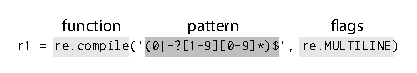
\includegraphics[width=\columnwidth]{../illustrations/exampleUsage.eps}
\caption{example of one regex utilization}
\label{fig:exampleUsage}
\end{figure}



\noindent \textbf{Pattern}: A \emph{pattern} is extracted from a utilization, as shown in Figure~\ref{fig:exampleUsage}. In essence, it is a string, but more formally it is an ordered series of regular expression language feature tokens.

Notice that because the vast majority of regex features are shared across most all-purpose languages, a Python {pattern} will (almost always) behave the same when used in other languages, such as Java, C\#, Javascript, or Ruby, whereas a utilization is not universal in the same way (i.e., it may not compile in other languages, even with small modifications to function and flag names).


% As an example, the {\tt re.MULTILINE} flag, or similar, is present in Python, Java, and C\#, but  the Python {\tt re.DOTALL} flag is not present in C\# though it has an equivalent flag in Java.
\todo{Carl: check the above paragraph}

In this work, we primarily focus on patterns since they are cross-cutting across languages and are the primary way of specifying the matching behavior for every utilization. Next, we describe the research questions and how the data set was collected and analyzed.

\subsection{Research Questions}
\label{sec:rqs}
Our overall research goal is to understand how regular expressions and regular expression features are used in practice. We aim to answer the following research questions:

\textbf{RQ1:} How  is the {\tt re} module used in Python projects?

To address this research question, we measure how often any calls are made to the {\tt re} module per file and per project in Python projects.

Furthermore, we measure the frequency of usage for calls to the 8 functions of the {\tt re} module ({\tt re.compile}, {\tt re.search}, {\tt re.match}, {\tt re.split}, {\tt re.findall}, {\tt re.finditer}, {\tt re.sub} and {\tt re.subn}) in Python projects scraped from GitHub.

We also measure usage of the 8 flags ({\tt re.DEFAULT}, {\tt re.IGNORECASE}, {\tt re.LOCALE}, {\tt re.MULTILINE}, {\tt re.DOTALL}, {\tt re.UNICODE}, {\tt re.VERBOSE} and {\tt re.DEBUG}) of the {\tt re} module.

Further, to provide context as to the overlap among regular expression strings used in Python, we explore the most common regex {patterns} across all utlizations.

\textbf{RQ2:} Which regular expression language features are most commonly used in python?

We consider regex language features to be tokens that specify the matching behavior of a regex pattern, for example,  the {\tt +} in {\tt ab+}.  All studied features are listed and described in Section~\ref{study:corpus} with examples.

To measure feature usage, we parse Python regular expression patterns using Bart Kiers' PCRE parser\footnote{\url{https://github.com/bkiers/PCREParser}}, as described in Section~\ref{study:corpus}.  We then count the number of usages of each feature per project, per file and as a percent of all distinct regular expression patterns.

\textbf{RQ3:} What is the impact of \emph{not} supporting various regular expression features on tool designers and users?
%\textbf{RQ3:} What is the impact of \emph{not} supporting various regex features on tool designers and users?

To address, this question, we use semantic analysis to illustrate the impact of missing features on a tool's applicability by identifying what each feature (or group of features) is commonly used for.

At a high level, our semantic analysis clusters regular expressions by their behavioral similarity. Behavioral similarity is determined by a pairwise comparison among all patterns. Within each pair, a set of strings is generated for each regular expression and then tested against the other. The average percentage of matching regular expressions creates the similarity level. By calculating pairwise similarity among all regex patterns, a similarity matrix is constructed for use during clustering.

\todo{Finish this example - I will get back to this next pass}
For example, consider the following two regular expressions, denoted A and B for reference.

\begin{verbatim}
state regex A
state regex B
\end{verbatim}

For each regex, the following strings are generated:

\begin{tabular}{l | l}
A & B \\ \hline
s1 & s2 \\
s3 & s4 \\
\end{tabular}

Each string in the A column matches regex A, and each string in the B column matches regex B. When testing the strings in B against regex A, X/5 = 0.Y\% match. When testing the strings in the A column against regex B, Z/5 = 0.W\% match. Thus, the similarity between these two regular expressions is 0.U\%.

To perform this similarity analysis on each pair of regex patterns, we use Rex for string generation.  We chose Rex to build matching strings because it supports the most features of any String-generation tool. To build the similarity matrix, we generated at least 384 strings per regular expression in an effort to balance the precision of the similarity metric (i.e., more strings lead to higher precision) with the speed of our analysis tool (i.e., more strings lead to longer runtimes).

Using the similarity matrix, clusters of regexes with similar behavior are discovered using Markov Clustering\footnote{\url{http://micans.org/mcl/}}.  These clusters are used to see how programmers implement regular expressions that match similar strings and interpret what a feature is used for.
 We chose the mcl clustering tool because it offers a fast and tunable way to cluster items by similarity and it is particularly useful when the number of clusters is not known \emph{a priori}.


Next, we describe in greater detail how the corpus of regex patterns was built, how features were analyzed, and how the clustering was performed.
%\todo{Is this still the case?}
%Since our semantic analysis is based on Rex, this semantic analysis cannot be applied to all features studied.  For these unsupported features, we use 6 string similarity metrics (Jaro-Winkler, Levenshtein, Longest Common Substring, Sift3, Jaccard and Cosine) to build similarity matrices.  As before, these matrices are used to find clusters of regexes, which are used to interpret what a feature is used for.




\subsection{Building the Corpus}
\label{study:corpus}
Github is a popular project hosting site containing over 100,000 Python projects.  The GitHub API assigns an integer identifier to each repository and can be used to clone relevant repositories for analysis.  Using the \url{http://api.github.com/repositories?since=N} interface page, we launched 32 scrapers to find repositories containing Python code.  The Github interface provides information about the first 100 repository IDs since the {\tt N} value on a single results page.  Each scraper used this information to identify repositories containing Python.  When a scraper was done with one page, it continued on to the next 100 repository IDs by using the interface again with {\tt N} now equal to the last repository ID on the current page.  Using this process, each scraper paged through the next available 1,000 repositories, cloning and scanning Python projects as they were found.  Each scraper started at a different {\tt N} value, with the first scraper starting at 0.  Scraper start indices were spaced by 262,144 so as to investigate within the first 8 million repositories.  At the time scraping was performed, the highest repoID was over 32 million, so we were cloning projects in the lowest fourth of the available space of IDs.  After this process was complete, \DTLfetch{data}{key}{nProjScanned}{value} Python projects had been cloned and scanned.

For each project, we used Astroid\footnote{\url{https://bitbucket.org/logilab/astroid}} to build the AST of each Python file and find utilizations of Python's {\tt re} module. This ensured that all utliizations of the {\tt re} module were captured for analysis.

Using git, each project's commit history was scanned at 20 evenly-spaced commits.  If the project had fewer than 20 commits, then all commits were scanned.  The most recent commit was always included, and the spacing between all other chosen commits was determined by dividing the remaining number of commits by 19 (rounding as needed).

Within one project, we define a duplicate utilization as a utilization having the same function, pattern and flags within the same file (same relative path).  We ignored duplicate utilizations across project versions to protect against over-counting the same utilization as we rewind the project through its history.  We observed and recorded \DTLfetch{data}{key}{nUsages}{value} non-duplicate regex utilizations in \DTLfetch{data}{key}{nProjScanned}{value} projects.

\subsection{Extracting Patterns}
As the focus of this study is regex features, our analysis targets the patterns. Thus,  we ignore the \DTLfetch{data}{key}{percentBadFlags}{value}\%  of utilizations using flags that can alter regex behavior.  An additional \DTLfetch{data}{key}{percentInvalidPattern}{value}\% of utilizations contained patterns that could not be compiled because the pattern was non-static (e.g., used some runtime variable), or because of other unknown parsing failures.

The remaining \DTLfetch{data}{key}{percentCleanUsages}{value}\% (\DTLfetch{data}{key}{nCleanUsages}{value}) utilizations were collapsed into \DTLfetch{data}{key}{nDistinctPatterns}{value} distinct pattern strings using sql.  Each of the pattern strings was pre-processed by removing Python quotes(\verb!'\\W!' becomes \verb!\\W!), unescaping escaped characters (\verb!\\W! becomes \verb!\W!) and parsing the resulting unescaped string using an ANTLR-based, open source PCRE parser released by Bart Kiers\footnote{\url{https://github.com/bkiers/pcre-parser}}.

This parser was unable to support \DTLfetch{data}{key}{percentUnicode}{value}\% (\DTLfetch{data}{key}{N_UNICODE}{value}) of the patterns due to unsupported unicode characters.  Another \DTLfetch{data}{key}{percentAlien}{value}\% (\DTLfetch{data}{key}{N_ALIEN}{value}) of the patterns used regex features that we have chosen to exclude in this study because they did not appear often enough (e.g., Reference Conditions).  The \DTLfetch{data}{key}{nCorpus}{value} distinct pattern strings that remain were each assigned a weight value equal to the number of distinct projects the pattern appeared in.  We  refer to this set of weighted, distinct pattern strings as the \emph{corpus}.

\subsection{Analyzing Features}
\label{study:features}
For each escaped pattern, the PCRE-parser produces a tree of feature tokens. Note that features such as capture groups or logical `OR' can contain sub-patterns composed of more tokens.  For each of these trees, we counted the number of tokens, creating a frequency-of-appearance vector or `\emph{featureCount}' for each pattern.  A pattern is said to contain a feature at an index if the value of the featureCount at that index is non-zero.

\todo{fill in this paragraph for a bridge between paragraphs}
For example, consider again the pattern in Figure~\ref{fig:exampleUsage}. This pattern has X different features, specifically, Y, Z, and W. The Y feature appears X times. The set if distinct fears forms the feature set for the pattern.

Once the feature set was established, we mapped the features from the corpus to those features supported by the four regular expression engines described in Section~\ref{sec:related}: brics, hampi, RE2, and Rex.
To create the tool mappings, we consulted documentation for each of the selected regular expression engines. For brics, we collected the set of supported features using the formal grammar\footnote{\url{http://www.brics.dk/automaton/doc/index.html?dk/brics/automaton/RegExp.html}}.  For hampi, we manually inspected the set of regexes included in the {\tt lib/regex-hampi/sampleRegex} file within the hampi repository\footnote{\url{https://code.google.com/p/hampi/downloads/list}} (this may have been an overestimation, as this included more features than specified by the formal grammar\footnote{\url{http://people.csail.mit.edu/akiezun/hampi/Grammar.html}}).  For RE2, we used the  supported feature documentation\footnote{\url{https://re2.googlecode.com/hg/doc/syntax.html}}.  For Rex, we were able to use trial and error because we tried to parse all patterns with Rex, and Rex provides good error feedback when a feature is unsupported.

\todo{Were there any features supported by the tools that we did not find in the corpus? Explain either way...tomorrow.  There are many, it seems less critical}
%Our semantic analysis is dependent on the use of Rex to generate strings so we can identify semantically related clusters. For three common features unsupported by Rex, we rely on syntactic analysis to determine similarity among regular expressions containing those features. For those features supported by Rex, we cluster the regular expressions based on semantic diversity.

\subsection{Clustering and Semantic Analysis}
We are interested in what behaviors users are trying to get when using regexes, and we know that the exact same behavior, or very similar behavior can be specified in many ways, as shown in Figure~\ref{fig:equivalentPatterns}. \todo{need to explain figure 2! guide the reader in understanding what figure 2 is illustrating - also inflate to just be an example of the actual process instead of a conceptual guide}

\begin{figure}[tb]
\centering
\fbox{
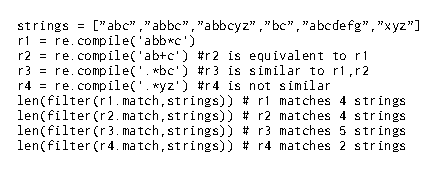
\includegraphics[width=\columnwidth]{../illustrations/equivalentPatterns.eps}
}
\caption{An Example of Patterns With Similar and Dissimilar Behavior}
\label{fig:equivalentPatterns}
\end{figure}

Rex can be used to generate a set of strings that will all match a pattern.  For each of the \DTLfetch{data}{key}{nCorpus}{value} distinct patterns, we use Rex to generate a set of at least 384 \emph{matching strings}. If fewer strings were generated, we did not include that pattern in the similarity analysis. The average number of generated strings per pattern was \todo{X} with a standard deviation of \todo{Y}. The maximum number generated was \todo{Z-these3:programming project for later tonight}.  The number 384 was selected to balance the runtime of the similarity analysis with the precision of the calculations. Since Rex does not support all the features present in the corpus, we could only generate sets of matching strings for 9,727 (70\%) of the \DTLfetch{data}{key}{nCorpus}{value} patterns in the corpus (omitted features are indicated in Table~\ref{table:featureStats} as described in Section~\ref{results:rq3}).

As explained in Section~\ref{sec:rqs}, we used these sets of matching strings to  measure the pairwise similarity between regular expressions and create a behavioral similarity matrix.  We will refer to a cell of this matrix with row index {\tt i} and column index {\tt j} as {\tt M[i][j]}.  For each pattern at index {\tt i}, we used Rex to create a set of matching strings which we will refer to as {\tt matching\_strings\_i}.  Then for every pattern at index {\tt j}, we set the value of {\tt M[i][j]} equal to the fraction of strings in {\tt matching\_strings\_i} that the pattern at index {\tt j} matched.

Once the matrix was complete, the values of cells reflected across the diagonal of the matrix were averaged to create a half-matrix of undirected similarity edges.  Using all similarity values in this half-matrix above 0.75, we created a text file specifying the edges of a graph.  This process is illustrated in Figure~\ref{fig:matrixToGraph}.
The first matrix represents \todo{explain}, the second matrix represents \todo{explain}, and finally the output is a file of the graph edges, \emph{out.abc}.
 Not that pairs DB and DC are omitted from the graph because their similarities are lower than the threshold.

\todo{Is the graph directed? Can you show the graph? how do the clusters emerge from the graph?}


\begin{figure}[tb]
\centering
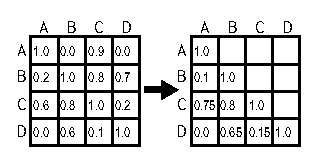
\includegraphics[width=\columnwidth]{../illustrations/matrixToGraph.eps}
\caption{Creating A Similarity Graph From A Similarity Matrix}
\label{fig:matrixToGraph}
\end{figure}


\todo{in progress!}

With 9,727 patterns there were 94,614,529 cells in the matrix, and although we were able to match them at a rate of about 8,300 cells per second, we had to save time by not

Markov clustering can be tuned using many parameters, including inflation and filtering out all but the top-k edges for each node.  After exploring the quality of the clusters using various tuning parameter combinations\footnote{\url{www.details.#thistopic}}, the best clusters were found using an inflation value of 1.8 and k=83.

There was an operational error in pulling  patterns from our database prior to the similarity analysis and clustering and 227 patterns (2.3\%) were omitted from the semantic analysis.

Note that the filteredCorpus is of size 9727, and at least one pattern from the fc can be found in 1375 of the original 3900 or whatever.  Most patterns do not belong in a cluster (for example a very specific pattern like \verb!<title>[^<]*Revision \d+:!), so after clustering is done only 2727 patterns are included, and only 999 projects have any of these patterns in them.

